\documentclass[notitlepage]{article}
\usepackage{color,soul,amsmath,graphicx}
\usepackage[outercaption]{sidecap}
\usepackage[citestyle=numeric,backend=bibtex]{biblatex}
\usepackage[font=small,labelfont=bf]{caption}
\usepackage{verbatim}
\sidecaptionvpos{figure}{c}
\providecommand{\abs}[1]{\lvert#1\rvert}
\providecommand{\norm}[1]{\lVert#1\rVert}
\bibliography{library}
\immediate\write18{python proteome-analysis.py}

\title{Increased concentration of proteins with growth rate can result from passive resource redistribution}
\author{Leeat Keren, Uri Barenholz, Ron Milo}

\begin{document}
\maketitle
\abstract{
  In many microorganisms, the proteome composition changes dramatically as a function of the growth environment.
Furthermore, many of these changes seem to be coordinated with the growth rate rather than the specific environment.
However, although cellular growth rates, gene expression levels and gene regulation have been at the center of biological research for decades, their quantitative interdependence is not yet fully understood.

We analyzed the relationship between growth rate and proteome composition for the model microorganism \emph{E.coli} as reflected in two recently published proteomics data sets spanning various growth conditions.
We found that the cellular concentration of a large fraction of the proteins measured coordinately increases with the growth rate.
This fraction includes proteins spanning different functional groups and proteins that are involved in different cellular processes.
Notably, ribosomal proteins are only a small fraction of this group of proteins.

We present a simple model that demonstrates how such a widely coordinated increase in the concentration of many proteins can be the result of passive redistribution of resources, due to active regulation of a few proteins.
Our model provides a potential explanation for why and how such changes relate to the growth rate under different environmental conditions.

In light of these results we conclude that, although the concentrations of many proteins change with the growth rate, such changes could be part of a global effect, not requiring specific cellular control mechanisms.
}

\section{Introduction}
A fundamental system-level challenge for cell physiology is the achievement of proper function in the face of various environmental conditions.
It has been established for many years that in different environments cells differ in many properties, including their shape, size, growth rate, and macro-molecular composition \parencite{Schaechter1958, Maaloe1969, Churchward1982, Pedersen1978a, ingraham1983growth,Bremer1987}, with strong interdependence between these parameters.

Early on it was found that the expression of some genes is coordinated with growth rate.
Classical experiments in bacteria, by researchers from what became known as the Copenhagen school, have shown that ribosome concentration (inferred from the RNA to protein ratio in cells) increases in proportion to growth rate\parencite{Schaechter1958}.
The search for mechanisms in \emph{E.coli} that underlie this observation yielded several candidates.
Specifically, coordination between ribosome production and growth rate was attributed both to the pools of purine nucleotides \parencite{Gourse1996,Gaal1997}, and the tRNA pools through the stringent response \parencite{Chatterji2001,Brauer2008a}.
For a more thorough review see \parencite{Nomura1984}.
The logic behind this observed increase is that, given that translation rates and ribosome occupancy ratios remain relatively constant across conditions, a larger fraction of ribosomes out of the biomass is needed in order to achieve faster growth \parencite{neidhardt1999a,dennis2004,Zaslaver2009}.

In the last two decades, with the development of the ability to measure genome-wide expression levels, it was found that coordination of protein concentration and growth rate is not limited to ribosomes and ribosomal genes, but is actually much more wide-spread.
In \emph{E.coli}, a coordination between the expression of catabolic and anabolic genes, and the growth rate, was observed, a process mediated by cAMP \parencite{Saldanha2004}.
In \emph{S.cerevisiae}, it was shown that a surprisingly large fraction of the genome changes its expression levels in response to environmental conditions in a manner strongly correlated with growth rate \parencite{Keren2013a,Gasch2000,Castrillo2007,Zaslaver2009, Berthoumieux2013, Gerosa2013}.
These studies and others raised many fundamental questions regarding the basic nature of gene regulation that are still open.
For example, what is the degree of interconnection between gene expression and growth rate? What are the mechanisms underlying this connection? Is it mostly due to specific mechanisms, each affecting a distinct group of genes (such as the mechanisms detailed above) or is it a more global phenomenon shared across most genes in the genome?

Several studies examining the interplay between global and specific modes of regulation tried to answer these questions, suggesting that global factors play a major role in determining the expression levels of genes \parencite{Gasch2000, Klumpp2009a,Scott2010}.
In \emph{E.coli}, this was mechanistically attributed to changes in the pool of RNA polymerase core and sigma factors \parencite{Klumpp2008}.
In \emph{S.cerevisiae}, it was suggested that differences in histone modifications around the replication origins \parencite{regenberg2006} or translation rates \parencite{Gasch2000} across conditions may underlie the same phenomenon.
Important advancements in understanding this process in \emph{E.coli} were achieved by coupling measurements of fluorescent reporters to a model of expression built upon the empirical scaling of different cell parameters (such as gene dosage, transcription rate and cell size) with growth rate \parencite{Klumpp2009a}.
These studies suggest that the expression of all genes change with growth rate, with different architectures of regulatory networks yielding differences in the direction and magnitude of these changes. 

Despite these advancements, many gaps remain in our understanding of the connection between gene expression and growth rate.
Importantly, whereas many of these studies depict gene expression as a function of growth rate, other studies suggest that the changes in expression temporally precede the changes in growth rate\parencite{levy2007}.
In addition, mechanistic insight and models for organisms other than \emph{E.coli} are still missing.
As such, a need remains for a quantitative model relating gene expression and growth rate, which can provide a baseline for the behavior of endogenous genes in conditions in which they are not differentially regulated.
Such a model will provide a basis on top of which different regulatory aspects can be added.

In this work we analyzed two recently published proteomic data sets of \emph{E.coli} under different growth conditions \parencite{Valgepea2013} [ref unpublished heinemann].
Based on the analysis we present a baseline, organism-independent model, that quantifies the relationship between gene regulation, protein abundance and growth rate.
Our model suggests that positive correlation with growth rate is a system-emerging property that is the result of passive redistribution of resources.
As a result, such an observed correlation does not require specific regulation of the positively correlated proteins and hence, no mechanism needs to exist in order to achieve this trait.

\section{Results}
\subsection{Analysis of proteomic data}
Having two high-quality data sets at hand, we looked for global trends in the data and specifically trends involving the growth rate under the different conditions analyzed.
We measured the Pearson correlation of every protein in the two data sets analyzed (denoted by H for Heinemann's data and V for Valgepea's data) against the growth rate (Figure \ref{fig:growthcorr}).
The two data sets present a large number of proteins ($724$ out of $1981$ measured in H and $296$ out of $2184$ in V) that are significantly positively correlated with the growth rate.
In the H data set, the correlation with growth rate is more significant among annotated proteins than among un-annotated proteins ($435$ out of $988$ of annotated proteins have a correlation in the range of $(0.4,0.8)$ whereas only $289$ out of $993$ of the un-annotated proteins have a correlation within this range).
In both data sets, the proteins that have a high correlation with the growth rate are involved in different cellular functions and span different functional groups (To-Do refer to table with breakdown by function).
We believe that the lower correlation and higher variability found in the H data set results from the fact that it contains much more conditions but spans roughly the same range of growth rates.
Furthermore, it includes measurements of the proteome under conditions involving different carbon sources as opposed to the V data set that uses the same carbon source on all measurements.
This is exemplified by restricting the analysis of the H data set only to chemostat conditions (Figure \ref{fig:growthcorrchemo}).
(To-Do consider discussing analysis with LB here or in the SI.)

\begin{figure}[h]
\centering
\includegraphics{GrowthRateCorrelation.pdf}
\caption{
A significant fraction of the proteins have positive correlation with the growth rate in the two data sets analyzed.
These proteins span all the functional groups.
Proteins with unknown function (present in the Heinemann data set, right panel) show less correlation with growth rate, as well as proteins with low levels of expression (data not shown).
}
\label{fig:growthcorr}
\end{figure}

Next, we checked how large is the response of the proteins that had a significant positive correlation with the growth rate across the conditions measured (referred to as HC, for High Correlation, proteins).
To that end, we summed up the concentrations of all of the HC-proteins across the conditions measured and compared their total concentration to the growth rate (Figure \ref{fig:globalgrcorr}).
Both data sets presented a significant response ($\approx 2$ fold change in total concentration across $\approx 5$ fold change of the growth rate) with most of the variability of the total concentration being explained by the growth rate ($R^2$ of $0.75$ in H and $0.99$ in V). 
As before, the H data set presented more noise, due to the reasons mentioned above (see Figure \ref{fig:growthcorrchemo} for analysis of the chemostat conditions of the H data set).

\begin{figure}[h]
\centering
\includegraphics{GlobalClusterGRFit.pdf}
\caption{
The sum of the concentrations of the HC proteins in each of the data sets (with linear regression lines) is shown.
HC proteins form a large fraction out of the proteome at higher growth rates ($>40\%$ for H and $>50\%$ for V).
The change in the concentration of the HC proteins is about 2-fold while the growth rate changes by about 5-fold.
Some of the unexplained variability of the HC proteins in the H data set can indicate errors in growth rate measurements and/or differences in degradation rates across conditions.
(HC proteins are defined as those with a Pearson correlation in the range $(0.4,0.8)$ and $(0.8,1)$ for the H and V data sets, respectively)
(To-Do: The estimated degradation rate is A for H and B for V (with confidence intervals).
}
\label{fig:globalgrcorr}
\end{figure}

Noting that the fact that two proteins have the same correlation with the growth rate does not imply that they are correlated between themselves, neither does it imply that they scale in the same way, we calculated the slope of a linear regression line with the growth rate for every protein in the HC proteins and plotted the results in Figure \ref{fig:globalfit}.
In order to compensate for the different concentrations of different proteins, the data for every protein was first normalized to have an average concentration of $1$ across the different conditions and then the slope of the fit was calculated.
The analysis reveals that most proteins respond in a similar manner to the different conditions.

Lastly, we wanted to check how the response of the HC-proteins relates to the well-studied response of the ribosomal proteins.
To that end, we performed the same analysis of slopes, restricting it to ribosomal proteins alone (Figure \ref{fig:globalfit}).
The analysis shows that, on average, HC-proteins scale in the same way as the ribosomal proteins do.

\begin{figure}[h]
\centering
\includegraphics{AllProtsVSRibosomalNormalizedSlopes.pdf}
\caption{
    A histogram of the normalized slopes of the trend lines for every protein in the HC proteins and for all the ribosomal proteins is shown for the two data sets analyzed.
    Left panel - Valgepea, Right panel - Heinemann.
    The HC proteins all share a relatively similar response, meaning they maintain their relative ratios.
    The ribosomal proteins respond in a similar manner to the HC proteins .
    (To-Do confidence intervals or some other heuristic for justifying the observed variation)
}
\label{fig:globalfit}
\end{figure}

\subsection{Theoretical model}
In an attempt to explain how such a wide-span positive response occurs, we have constructed a minimalistic model that is able to reproduce these results as the outcome of redistribution of resources of the bio-synthesis machinery.
Briefly, the model assumes that favorable growth conditions allow the cell to down-regulate some proteins that are needed in harsher conditions, thus reducing the amount of proteins that need to be produced for the cell to proliferate (Figure \ref{fig:model}).
As a consequence, the fraction of each of the rest of the proteins out of the proteome increases, assuming they are being expressed in the same relative ratios, without invoking specific regulation.
The growth rate therefore increases as well, due to the fact that the ratio of bio-synthetic machinery to the rest of the proteome increases.

\begin{figure}[h]
\centering
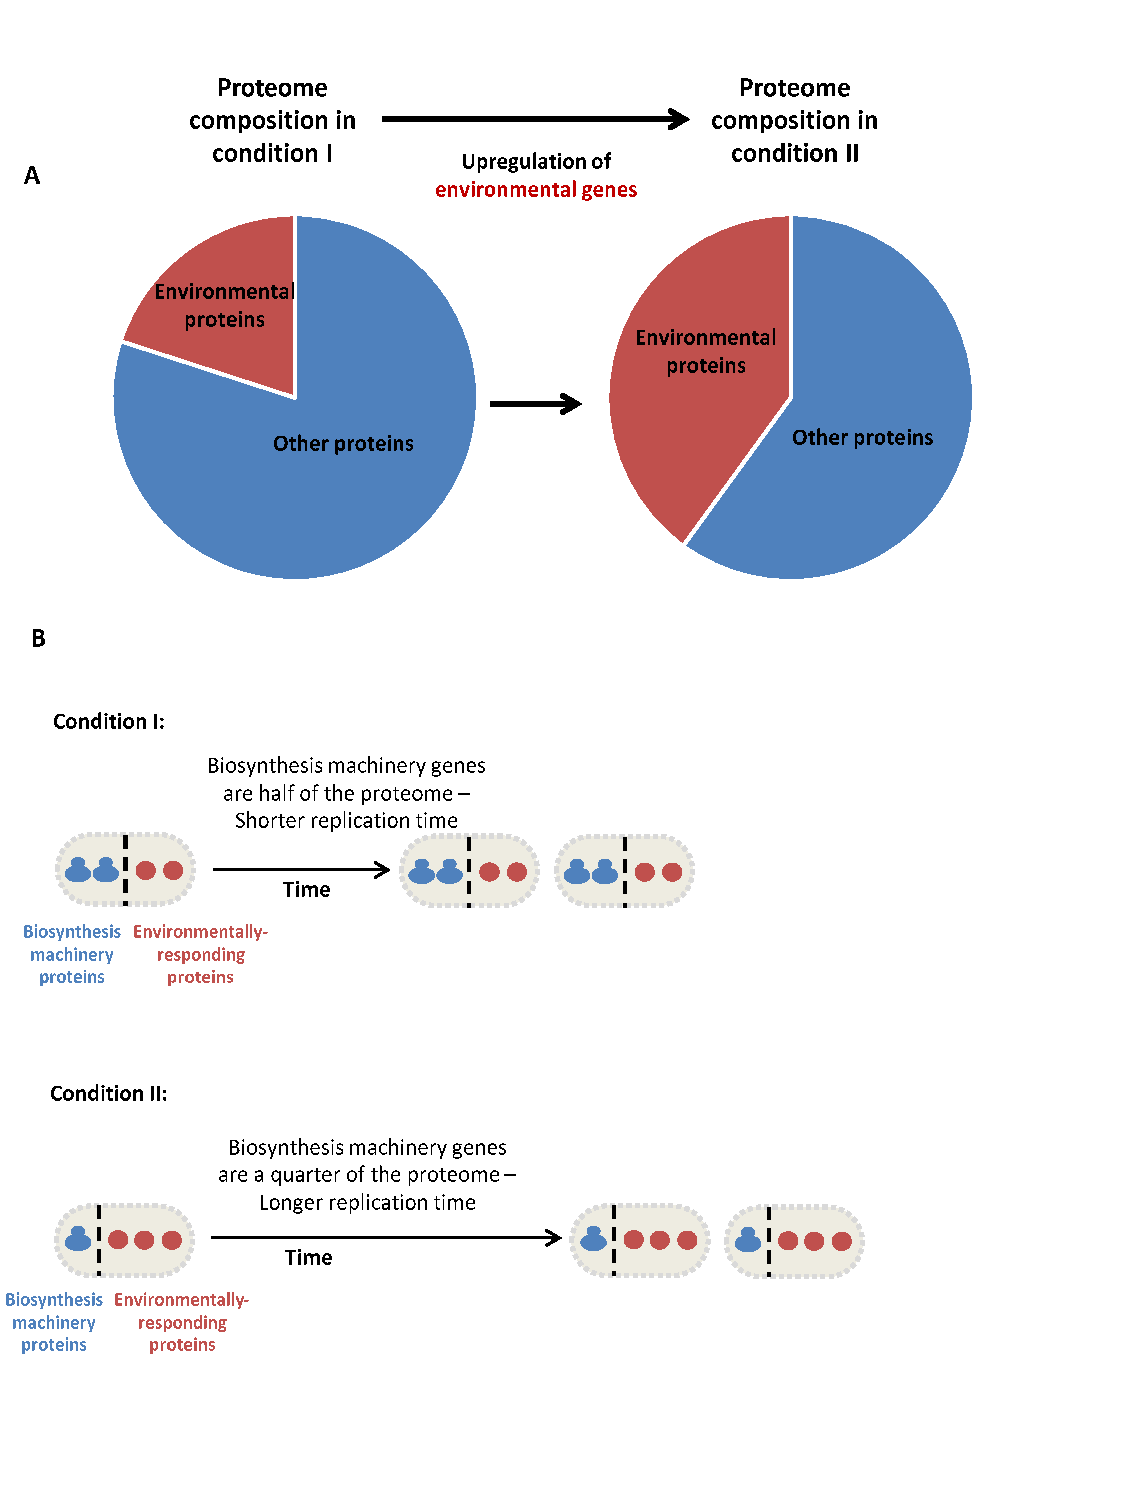
\includegraphics[scale=0.8]{Figures7-trieste.pdf}
\caption{
  A minimalistic model predicts up regulation of environmental genes reduces the concentration of other proteins (Panel A).
As a result, the ratio of bio-synthesis machinery genes to the rest of the proteome decreases, resulting in slower growth (Panel B).
}
\label{fig:model}
\end{figure}

\subsubsection{Distinguishing between gene specific and global control of expression}
For every protein, the model decouples its resulting concentration as the product of two control mechanisms:
\begin{enumerate}
\item Protein/gene specific controls such as the associated gene's promoter sequence, 5'-UTRs, ribosomal binding site sequence, and factors affecting this specific gene's expression such as transcription factors and riboswitches that react with the relevant gene.
  While some of these controls (such as, for example, the 5'-UTRs) are static, and therefore condition independent, others are dynamic and may differ under different environmental conditions (such as transcription factors state).
\item The global state of the cell, including availability of RNA Polymerase, co-factors, Ribosomes, amino-acids etc.
\end{enumerate}
According to the model, every gene, under every environmental condition, is given an 'affinity-for-expression' (or 'intrinsic-strength') score that encapsulates its gene-specific control state under the condition considered (denoted $w_i(c)$, where $c$ refers to the growth condition).
Our model assumes that the bio-synthetic resources of the cell (Ribosomes, RNA Polymerases, etc.) are distributed among the genes according to their affinities under the condition at hand.
The resulting protein concentration, under a specific condition, is therefore its specific affinity under the condition, divided by the sum of all the affinities of all of the genes under that same condition.
Thus, if two proteins have the same affinity under some condition, they will have the same concentration under that condition, if protein $A$ has twice the affinity of protein $B$ under the same condition, then $A$'s concentration will be twice as high as $B$'s concentration under that condition, etc.

This relationship can be simply formulated as follows:
\begin{equation}
  \label{eq:concentration-ratio}
  p_i(c)=\frac{P_i(c)}{P(c)}=\frac{w_i(c)}{\sum_jw_j(c)}
\end{equation}
where $p_i(c)$ denotes the concentration of protein $i$ under condition $c$, $P_i(c)$ denotes the mass of protein $i$ under condition $c$ per cell, and $P(c)$ denotes the total mass of proteins per cell under condition $c$).

\subsubsection{How different growth conditions reflect in the proteome composition}
Different environmental conditions may require the expression of different genes in order to achieve growth.
For example, comparing two growth media, one that includes all the required amino-acids (abbreviated as AA), and one that includes none, it can be assumed that when all the AA are present, no need exists for the cell to express AA metabolism enzymes, whereas when AA's are absent, these enzymes must be expressed.
If we now consider some arbitrary protein $i$, whose specific affinity is unaltered between these two conditions, we see that its concentration will most likely still change between the two conditions as the affinities of at least some of the genes (the AA synthesizing enzymes) change, affecting the distribution of resources between all of the expressed genes.

Generalizing this notion, for every group of conditions, one could divide the proteins into those whose intrinsic affinity remains constant across all of the conditions, and to those whose intrinsic affinity changes (meaning their expression is actively regulated by the cell) between at least some of the conditions.
As an outcome of Equation \ref{eq:concentration-ratio} it follows that those proteins whose intrinsic affinity remains constant across the different growth conditions, also maintain their relative concentrations across these conditions with respect to each other.
Therefore, identifying a large group of proteins that maintain their relative concentrations across conditions may indicate that these proteins maintained their intrinsic affinities and that any changes in their absolute concentrations are in fact a passive outcome resulting from changes in the intrinsic affinities of other proteins.

\subsubsection{The relationship between proteome composition and the growth rate}
While it is sometimes implied that different cellular components are regulated by the growth rate, here we treat the growth rate as an outcome of the combination of proteome composition and the environmental conditions.
Specifically, we evaluate the growth rate as the result of dividing the total amount of proteins per cell by the amount of bio-synthesis machinery in that cell.
The larger the ratio of total proteins to bio-synthesis proteins is, the longer these bio-synthesis proteins will have to operate in order to duplicate the proteome, and thus the longer the doubling time of the cell will be.

To illustrate this assumption concretely, one could think about the total amount of proteins per cell (measured in AA count) divided by the number of ribosomes in the cell.
As each Ribosome translates at an approximately condition-independent rate of about 20 AA per second, and as the amount of actively translating Ribosomes is also relatively condition-independent (refs), it follows that the doubling time is linearly dependent on the ratio of proteins to ribosomes in the biomass.

Theoretically, the fastest doubling time a cell may have is the doubling time achieved when all of the cell's proteome is the bio-synthetic machinery.
We denote this minimal doubling time by $T_B$.

To integrate the notion of total protein to bio-synthetic protein ratio into our model, we assume that there is a group of bio-synthetic genes (e.g. genes of the transcriptional and translational machineries) which are not differentially regulated across different conditions.
Furthermore, we assume that the machineries these genes are involved at operate at relatively constant rates and occupancy ratios across conditions.
Mathematically we can therefore define this group of bio-synthesis genes, $G_B$, such that, for every gene that belongs to this group, its affinity is constant regardless of the condition:
\begin{equation}
  \label{eq:biosynth-def}
  \forall k \in G_B, c \rightarrow w_k(c)=w_k
\end{equation}

To keep our notations short, we will define the (condition independent) sum over all of these genes as the constant: $W_B = \sum_{k\in G_B}w_k$.

As these genes form the bio-synthesis machinery, and according to the logic presented above, it follows that the doubling time under a given condition, $\tau(c)$ will be linearly proportional to the ratio of total protein to bio-synthesis protein under that condition, with the proportionality constant being $T_B$:
\begin{equation}
  \label{eq:gr-ratio}
  \tau(c) = T_B\frac{P(c)}{\sum_{k\in G_B}P_k(c)}=T_B\frac{\sum_jw_j(c)}{W_B}
\end{equation}
Therefore, the model implies that for conditions that require the expression of larger amounts of non-bio-synthetic genes, the resulting doubling time will be longer, and thus, the growth rate will be lower.

\subsubsection{The concentration of a non-differentially regulated protein is expected to increase with the growth rate} 
Recalling that the connection between the growth rate and the doubling time is: $g(c)=\frac{\ln(2)}{\tau(c)}$, we now combine Equation \ref{eq:concentration-ratio} with Equation \ref{eq:gr-ratio} to get that:
\begin{equation}
  \label{eq:default-response}
  p_i(c)=\frac{w_i(c)}{\sum_jw_j(c)}=\frac{w_i(c)}{W_B}\frac{W_B}{\sum_jw_j(c)}=\frac{w_i(c)}{W_B}\frac{T_B}{\ln(2)}g(c)
\end{equation}

Incorporating all the condition-independent constants ($W_B$, $T_B$, $\ln(2)$) into one term, $C$, we get that the predicted concentration of protein $i$ under condition $c$ is:
\begin{equation}
  \label{eq:final-conc}
  p_i(c)=Cw_i(c)g(c)
\end{equation}
which implies that, for every two conditions between which $i$ maintains its affinity, $i$'s concentration will scale like the growth rate change between these two conditions.

\subsubsection{Accounting for protein degradation}
Thus far, our model neglected the effect of protein degradation.
Our model also predicted that, for non-differentially regulated proteins, their concentration should drop to 0 when the growth rate is 0.
Interestingly, protein degradation affects the expected concentration of non-differentially regulated proteins at 0 growth rate.

Assuming that protein degradation acts on all proteins in the same way, and that it is invariant in the growth rate, the effect of protein degradation can be understood as follows: at any time, some fraction of the entire proteome is degraded.
Therefore, the \emph{observed} growth rate, $g$, is, in fact, the amount of proteins produced minus the amount of proteins degraded.
To illustrate, if the measured growth rate is 0, the implication is not that no proteins are produced, but rather that proteins are produced at exactly the same rate as they are degraded.

Integrating this notion into the model means that, where the equations previously referred to the observed growth rate, $g$, as the indicator of protein synthesis rate, they should in fact refer to the observed growth rate plus the degradation rate, as that is the real rate of protein synthesis.
Therefore, if we denote by $\alpha$ the degradation rate, Equation \ref{eq:final-conc} should be rewritten as:
\begin{equation}
  \label{eq:final-conc-deg}
  p_i(c)=Cw_i(c)(\alpha+g(c))
\end{equation}
which now yields much better agreement with the experimental results as presented in Figure \ref{fig:globalgrcorr} and explains why the concentration of non-differentially regulated proteins does not drop to 0 when the growth rate is 0.
\section{Discussion}
We identified a significant, coordinated correlation between many proteins and the growth rate.
This response spans proteins from various functional groups and is not related to the specific medium of growth.
We presented the notion of intrinsic affinity for expression and the limited bio-synthesis capacity as factors that, combined, can explain the response observed in the experimental data.
We note that the notion of affinity for expression was first presented in \parencite{Maaloe1969}.
However, only recently did experimental data made the exploring this idea possible.

Other works have suggested different models and in some cases have results that do not coincide with those presented in this work.
Notably, in \parencite{Klumpp2009a} the opposite behavior for unregulated gene is predicted.
We note that, among the reasons that could explain this discrepancy are the different ranges of growth rates observed in these two works, as well as the different ways by which the expected behavior is deduced.

Many works monitored the ribosome concentration in cells \parencite{Scott2010, Bremer1987, Schaechter1958, 1974, eco-sal} and in some cases had different expected response strengths than those observed in this work.
These differences can result, again, from the different growth rates monitored.
Moreover, these works deduced the amount of ribosomes by measuring the RNA to protein ratio, assuming a relatively fixed portion of the RNA is rRNA.
In this work, in contrast, ribosomal proteins are measured.
Therefore, and as it is known that ribosomes can operate even in the absence of some ribosomal proteins, such differences in manner of inference can account for some of the differences encountered.

While our work assumes that many bio-synthesis rates are condition independent, that may not be the case under specific kinds of conditions.
Specifically, changes in temperatures, osmotic pressure and PH levels may change such rates.
Slow growth rates, or cells at stationary phase, may also present different bio-synthesis rates.
In our analysis of data, we therefore considered only conditions for which this assumption will likely hold.
Importantly, we have omitted from the Heinemann data set stationary conditions and heat, PH and osmotic stress conditions.
Analysis of these conditions is provided in the SI.

As, out of the conditions measured in the Heinemann data set, growth in LB media presented a much faster growth rate than the rest of the conditions measured, it dominated the behavior and trends calculated.
We have therefore omitted it as well to allow for a more statistically robust analysis.
The analysis of growth in LB is presented in the SI.

The definition of protein concentration, or protein fraction out of the proteome is somewhat elusive.
One could consider the number of molecules of a specific protein out of the number of molecules of all of the proteome, or, alternatively, the mass ratio of one protein to the mass of the entire proteome.
We use the mass ratio as we find it to better represent the meaning of a fraction out of the proteome.
However, we note that if initiation rates are limiting, and not elongation rates, then using molecule counts may be a better metric.
We compared these two metrics and, while they present some differences in the analysis, these differences are marginal (see SI for comparison).

Our model demonstrates that no specific control mechanisms need to exist in order to achieve a linear correlation between ribosomal proteins and the growth rate.
However, many such mechanisms have been described before(refs).
We stress that the model does not contradict the existence of such mechanisms.
They may still be needed to achieve faster response under changing environmental conditions or a tighter regulation to avoid unnecessary production and reduce translational noise.
However, the fact that many non-ribosomal proteins share the same response poses interesting questions regarding the scope of these control mechanisms, their necessity and the trade-offs employing them present.

\section{Materials and Methods}
Detail data sources, software and algorithms used.

\section{Supplementary figures and data}
\begin{figure}[h]
\centering
\includegraphics{HeinmannChemostatGr.pdf}
\caption{
  Restricting the analysis of the Heinemann data set to chemostat conditions yields similar results to those of the Valgepea data set.
}
\label{fig:growthcorrchemo}
\end{figure}

\begin{comment}
\begin{figure}[h]
\centering
\includegraphics{CoordinatedRSquareComparison.pdf}
\caption{
  Proteins in the global cluster fit reasonably well to the global cluster itself
}
\label{fig:globalfit}
\end{figure}

\begin{figure}[h]
\centering
\includegraphics{GlobalClusterCorr.pdf}
\caption{
Proteins that have a high correlation (0.4-0.8) with growth rate mostly have even higher correlation to the sum of these proteins (both weighted sum and normalized sum are presented).
Weighted sum means the concentrations of all proteins in the group are summed.
Normalized sum means every protein is first normalized to have an average concentration of 1 across the different growth conditions, and then all proteins in the group are summed.
The higher correlation indicates that their response is coordinated (they scale by the same factor between conditions).
}
\label{globalcorr}
\end{figure}

\begin{figure}[h]
\centering
\includegraphics{GlobalClusterRSquare.pdf}
\caption{
Plotting the $r^2$ distribution shows that a large fraction of the variability of these proteins is captured by the global response.
}
\label{globalrsq}
\end{figure}

\end{comment}
\printbibliography
\end{document}
%%% LaTeX-command: "pdflatex -enable-write18"